Per \textit{servizio di visualizzazione di carte geografiche} si intende un sistema, disponibile in rete, che permette l'utilizzo e la consultazione di mappe geografiche. Nel corso di questo capitolo verrà illustrato il funzionamento e le caratteristiche principali dei maggiori competitor del settore.

\section{OpenStreetMap}

\textbf{OpenStreetMap (OSM)} è molto più di un semplice servizio di visualizzazione di mappe, volendo citare proprio la comunità che ha creato e gestisce il progetto: "OpenStreetMap is a map of the world, created by people like you and free to use under an open license" (\textit{OpenStreetMap è una mappa del mondo, creata da persone come te e utilizzata sotto licenza libera}).\cite{OSM}


\textit{OSM}, come si può capire dalla citazione, è un progetto sviluppato e realizzato da una comunità di persone. Fondato nel 2004 da Steve Coast con lo scopo di creare una mappa libera del mondo, nel 2006 ebbe inizio il processo per la trasformazione della società in fondazione non a scopo di lucro, da cui anche la rinominazione in \textbf{OpenStreetMaps Foundation}.

La \textit{"mappa"} negli anni ha subito diverse modifiche e soprattutto è cresciuta grazie alle donazioni non solo di utenti privati, ma sopratutto di enti e aziende quali ad esempio \textit{Automotive Navigation Data}, che nel 2007 donò il database stradale completo dei Paesi Bassi e quello delle principali strade di India e Cina.

La particolarità e l'unicità di questo progetto è sicuramente la sua licenza. Il database è pubblicato secondo la \textit{Open Database License}, la licenza che permette di condividere e adattare il database e creare opere a partire dallo stesso. Le uniche condizioni da rispettare secondo la \textit{ODbL} sono:
\begin{itemize}
\item attribuire l'appartenenza del database ad ogni suo utilizzo e ad ogni utilizzo di una banca dati derivata;
\item se viene pubblicato il database con una modifica rispetto all'originale o si creano nuovi database a partire da esso è obbligatorio distribuire il nuovo database secondo la licenza \textit{OBdL};
\item anche se il database venisse redistribuito in una nuova versione che ne restringa la libertà d'utilizzo, deve rimanere disponibile una versione aperta del database priva delle restrizioni.
\end{itemize}

Allo stesso modo del database, anche i dati inseriti e caricati dagli utenti devono rispettare una licenza compatibile con la Creative Commons e gli stessi contributori devono essere registrati al progetto.

Le modifiche operate sulla mappa vengono registrate in un elenco visibile sul sito web della fondazione, come visibile nella figura \ref{fig:OSMchangesets}.

\begin{figure}[H]
	\centering
		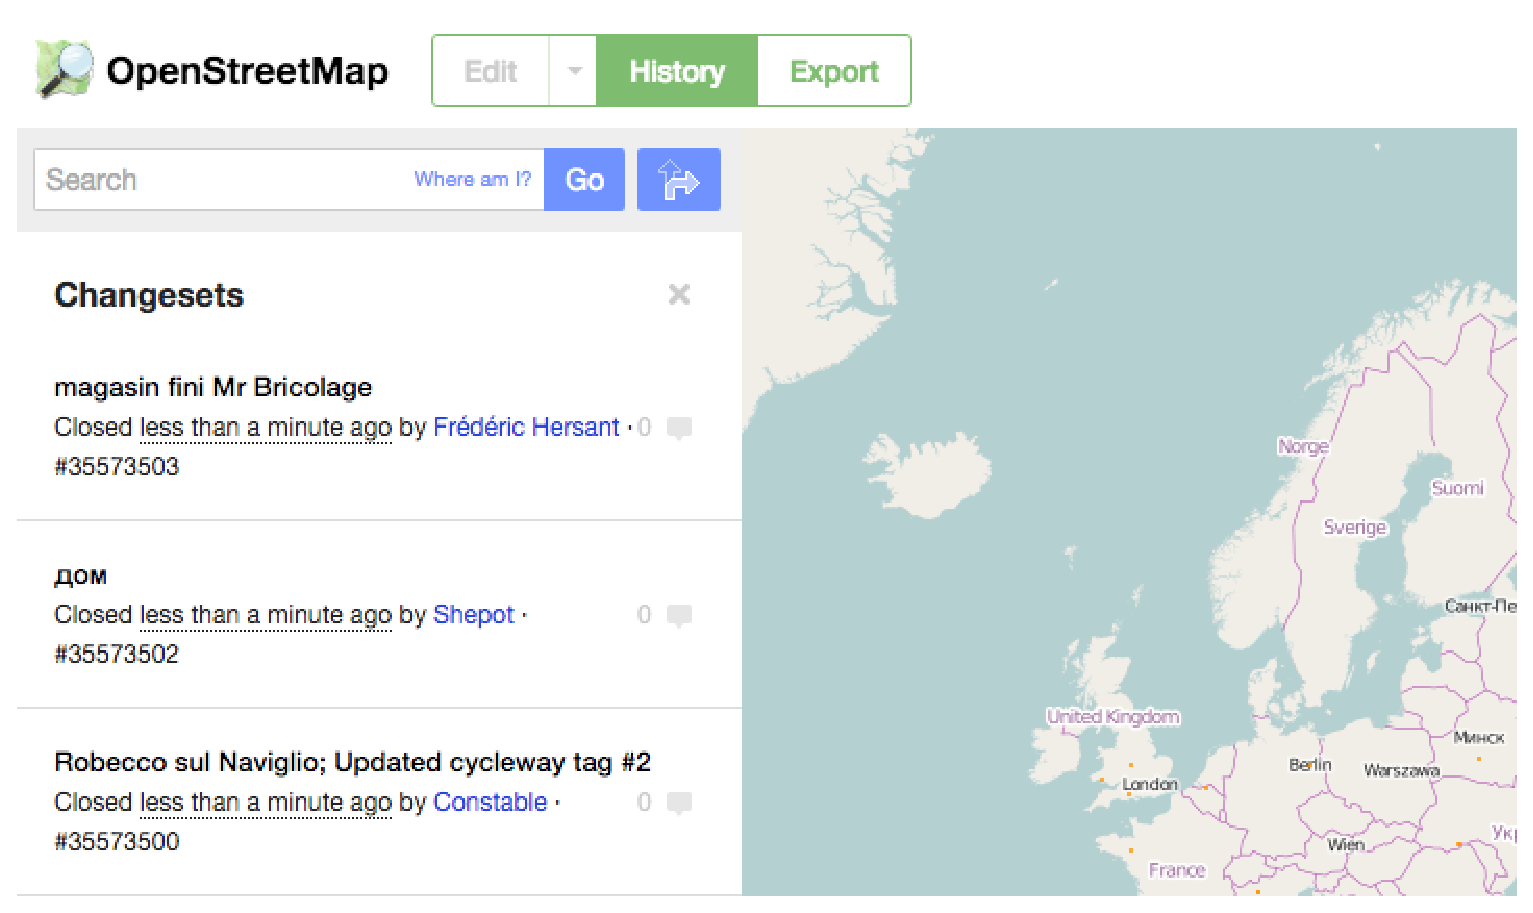
\includegraphics[scale=0.5]{figure/OSMchangesets.eps}
	\caption{Records di modifica della mappa ad opera di utenti} \label{fig:OSMchangesets}
\end{figure}


I dati di \textit{OpenStreetMap} sono utilizzati inoltre da uno dei principali provider di questo settore, ovvero \textbf{Mapbox}. L'utilizzo di quest'ultimo lo abbiamo inconsciamente visto diverse volte navigando su internet, su siti web come \textit{Foursquare}, \textit{Pinterest}, \textit{Evernote}, \textit{Financial Times} e \textit{National Geographic}.\cite{mapbox:showcase}

\section{Bing Maps}

Dopo aver visto un servizio \textit{open source}\footnote{Open Source\cite{wiki:opensource}} come \textit{OSM}, è importante vedere anche il competitor forse più \textit{"demonizzato"} dal mondo delle licenze libere. Infatti in questa sezione, descriveremo il funzionamento e le caratteristiche di Bing Maps, il sistema di \textit{web mapping}\footnote{Con "Web Mapping" si intende il processo di utilizzo o offerta di mappe sul World Wide Web} di creato e sviluppato dalla Microsoft.

In questo servizio a differenza di \textit{OpenStreetMap} le mappe non sono curate da una comunità di developer ma raccolte ed elaborate in diversi modi. Anche Bing Maps come \textit{Mapbox} attinge ai database di OSM per le mappe stradali, che rappresentano la visualizzazione di default. È necessario però sottolineare che, a differenza dei due servizi sopra citati, quello di Microsoft offre altre possibilità di visualizzazione delle cartine, consentendone anche una vista aerea, una cosiddetta "\textit{bird's-eye view}" (vista a volo d'uccello, che ne permette una proiezione grafica su un piano ortogonale), una veduta stradale che consente di vedere la strada a 360 gradi e infine troviamo la possibilità di accedere a mappe 3D in cui a prendere forma, oltre ai terreni e alle montagne, ci sono anche palazzi e monumenti. Di seguito vengono illustrati alcuni esempi di visualizzazione delle mappe di Bing:

\begin{figure}[ht]
	\centering
	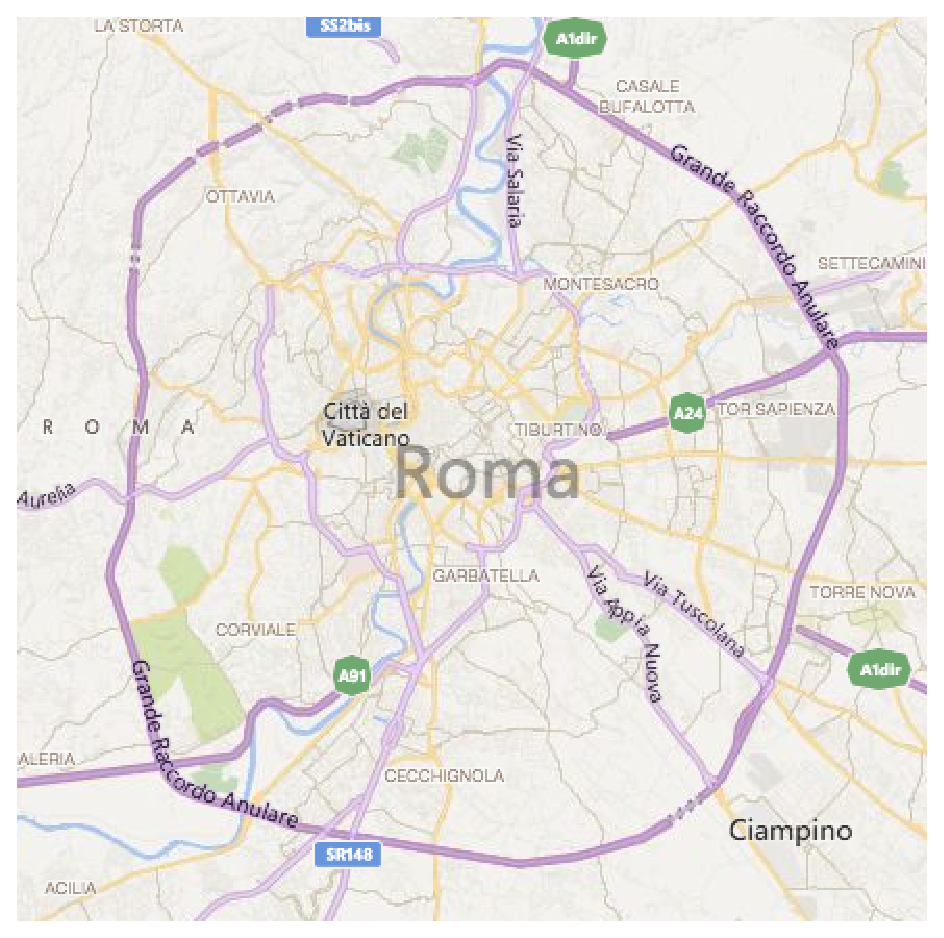
\includegraphics[scale=0.4]{figure/BINGRoadmap.eps}
	\caption{Esempio di mappa stradale di Bing}\label{fig:BINGRoadmap}
\end{figure}

\begin{figure}[ht]
	\centering
	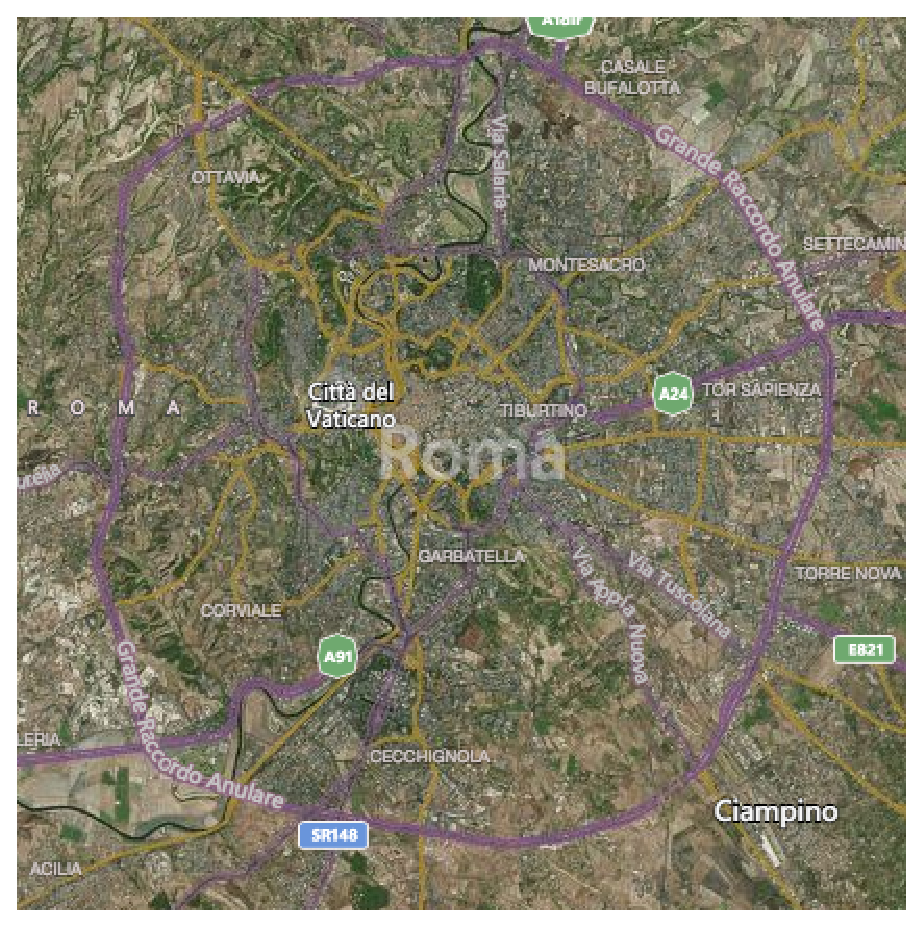
\includegraphics[scale=0.4]{figure/BINGAerial.eps}
	\caption{Esempio di mappa aerea di Bing}\label{fig:BINGAerial}
\end{figure}

\begin{figure}[H]
	\centering
	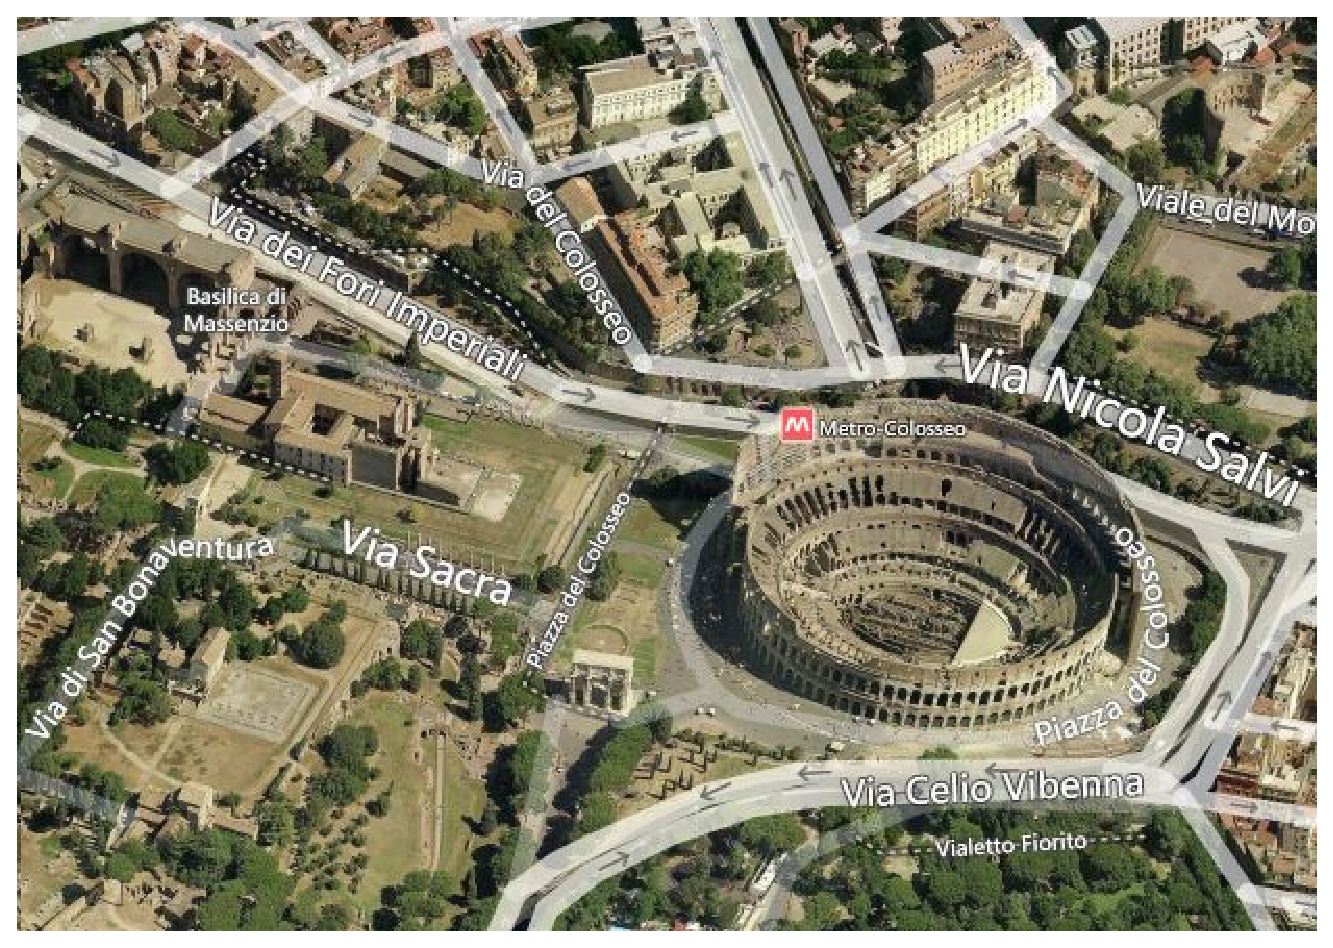
\includegraphics[scale=0.5]{figure/BINGBirdseye.eps}
	\caption{Esempio di visualizzazione Bird's-eye}
\end{figure}

Una delle peculiarità probabilmente più interessanti di Bing Maps, comunque, è la presenza al suo interno di differenti "Map Apps" delle vere e proprie applicazioni interne al servizio che ne sfruttano funzionalità e informazioni e ne arricchiscono così anche l'esperienza d'uso da parte dell'utente finale. Per fornire un esempi di questo utilizzo, si può far riferimento all'edizione del 2010 del \textit{Tour de France} che utilizzava la mappa Bing per mostrare risultati e tracciati delle differenti tappe della nota competizione ciclistica.\cite{bing:tdf}

\section{Google Maps}